% \documentclass[conference]{IEEEtran}
\documentclass[font=12pt]{article}
\usepackage{graphicx}
\usepackage{algorithm}
\usepackage{algorithmic}
\usepackage{amsmath}
\usepackage{flushend}

\DeclareGraphicsExtensions{.pdf, .jpeg, .png, .jpg}
\graphicspath{{images/}}

\title{Deep Learning:\\ A Review of the State of the Art}
\author{Luke Fraser\\
University of Nevada, Reno}
\begin{document}
\maketitle
\begin{abstract}
In this assignment we will summarize the uses and work of \emph{Deep Neural Networks}. Deep leaning has produced promising results for machine learning. Training large networks on difficult classification problems has produced machines that are capable of human levels of classification for the first time. These networks are complex and training deep networks comes with many challenges. This paper will provide a brief look at the state of the art in deep learning methods and applications in image classification.
\end{abstract}

\section{Introduction}
Deep neural networks have grown in popularity in the past few years as training sets have increased in size and computer hardware has allowed for larger and more complex networks \cite{krizhevsky2012imagenet,sanchez2011high,6248110}. These networks deal with large input datasets and a large number of classification classes. The main challenges of deep learning are defined in the following subsections.
\subsection{Storage}
Managing the large datasets required to train modern machine learning approaches is challenging. Recently there has been a lot of effort in producing large labeled datasets \cite{deng2009imagenet,Torralba:2008:MTI:1444381.1444403}. These datasets are very large. Storing the full ImageNet\cite{deng2009imagenet} dataset would take around 23TBs of storage \cite{sanchez2011high}. Such storage is not feasible on any standard hardware. A long with the soring this data when training with such large datasets other challenges manifest themselves. Common large storage mechanisms can not keep up with the CPU needs of a system. This means that while training the most costly aspect of the training is reading and writing data, rather than the cost of the actual training.

To deal with storage limitations methods of dimensionality reduction have been used. The goal of these methods is to reduce the size of the data input into the classifier to prevent dealing with very high dimensioned data. As well these reduction in size can increase the speed of the classification significantly. This speed up becomes significant when dealing such large datasets and high dimensionality of the data.

\subsubsection{Dimensionality Reduction}
Reducing the dimensionality of the problem is a popular method for dealing with high dimensional data. Image classification is a common case when dimensionality reduction is critical. Images can have millions of pixels and inputting this data to a classifier can quickly become a non-tractable problem on modern day hardware.

Dense projection techniques are among the most popular methods for dimensionality reduction. Principal Component Analysis (PCA), Partial Least Squares (PLS), and Gaussian Random Projections (RPs) are a few common methods used to project data to lower dimensions \cite{sanchez2011high}. The computational cost of performing these methods is proportional to the input and output dimensions. These methods are well suited when the input dimension is high and the output dimension is small. When small inputs are used on classifiers the performance diminishes with large output classes. Hash kernels were proposed to deal with this problem \cite{shi2009hash,weinberger2009feature}. Hash kernels have been used to compress text features \cite{shi2009hash,weinberger2009feature}.

\subsubsection{Summary}
Overall there is a trade off between storage and accuracy as well as computational cost. It is important to understand the trade offs and control the input to the system to produce acceptable results.

\subsection{Memory}
Memory is another limiting factor for many deep learning networks. Memory puts a hard limit on the number of neurons that can fit on a computers memory. A lot can be gained from having large networks as more complex training and accuracy can be achieved \cite{krizhevsky2012imagenet}. In \cite{krizhevsky2012imagenet} a large neural network was placed onto two 3GB GPUs. The size of the network was dictated by number of connection and the number of neurons that could fit on each of the GPUs. 

\subsection{Computational Cost}
The computational complexity of machine learning methods is a constant limiting factor in the speed and accuracy of classification. Deep learning relies heavily on new computer hardware to produce usable classifiers. Deep learning networks are very large and have many parameters that require increasing amounts of computation time to produce trained classifiers. Modern deep learning networks can take weeks, months, and even years to train on modern CPUs \cite{6248110}. New hardware options such as GPUs have been used to address these issues. Care must be taken in the design of the networks that are to be trained in order to produce a network that can train in a reasonable amount of time. These design decisions come in two forms hardware considerations and algorithm considerations. Many approaches take advantage of modern hardware and algorithms to produce highly accurate classifiers \cite{6248110,krizhevsky2012imagenet,sanchez2011high,long2015fully}.

\subsubsection{Hardware}
GPUs recently have been used to address long training times. They have brought training times down to reasonable durations, hours, days, and weeks. With the use of GPUs network can train on larger deep networks faster. Neural networks involve many parallel operations. A CPU does not take advantage of a Neural networks inherently parallel computations. A CPU is more capable of handling sequential tasks. The GPU has the advantage of performing millions of parallel operations as is necessary for graphics applications. This capability allows for 50-100 times speedup when compared to a CPU \cite{6248110}. 

\subsubsection{Algorithm}
Aside from hardware opportunities algorithmic decisions have a much larger effect on the training time and runtime of a given classifier. This can be seen in the choices of \emph{activation functions}. Section~\ref{sec:activation} will describe the effects of different activation functions in detail.

\section{Activation Functions}
\label{sec:activation}
The activation functions of a given layer of a deep network can determine the tractability of the training of the classifier. There are trade-offs between computation time and trained accuracy of different \emph{activation functions}. The main trade-off is seen between linear and non-linear activation functions. A linear activation function significantly limits the capabilities of the classifier as a linear classifier is best for representing linear problems. In the case of most interesting classification problems are non-linear which makes the use of the linear activation functions extremely limiting as they can not be used to represent an arbitrary function. In the case of a non-linear activation function a two layer neural network can be proven to be a universal function approximator \cite{cybenko1989approximation}. This means that non-linear activation function are more powerful and general than their linear counterparts.

A limitation of non-linear activation functions comes in the form of computational complexity. Linear activation functions are of low-cost compared to non-linear ones. The result of using either is a trade-off between accuracy and computational complexity. Current approaches deal with the trade-offs using a hybrid approach. Some of the layers in a neural network have non-linear activation functions and other have linear functions. An example of such a network is in \cite{krizhevsky2012imagenet}, where they use a softmax, logistic regression, and ReLU in deep learning network. As well, in \cite{6248110} they use a hyperbolic tangent, linear, and softmax for their deep learning network. The following function are a list of notable activation functions:

\begin{itemize}
\item identity:
\begin{equation}
f(x) = x
\end{equation}
\item Binary Step:
\begin{equation}
f(x) =
\begin{cases}
0 & if~x < 0\\
1 & if~x \geq 0
\end{cases}
\end{equation}
\item Logistic:
\begin{equation}
f(x) = \frac{L}{1 + e^{-k(x - x_0}}
\end{equation}
\item TanH (Hyperbolic Tangent):
\begin{equation}
f(x) = \frac{2}{1+e^{-2x}} - 1
\end{equation}
\item Rectified Linear Unit (ReLU):
\begin{equation}
f(x) =
\begin{cases}
0 & if~x < 0\\
x & if~x \geq 0
\end{cases}
\end{equation}
\item Exponential Linear Unit (ELU):
\begin{equation}
f(x) =
\begin{cases}
\alpha (e^x -1) & if~x < 0\\
x & if~x \geq 0
\end{cases}
\end{equation}
\item Sinusoid:
\begin{equation}
f(x) = sin(x)
\end{equation}
\item Sinc:
\begin{equation}
f(x) =
\begin{cases}
1 & if~x=0\\
\frac{sin(x)}{x} & if~x \neq 0
\end{cases}
\end{equation}
\item Gaussian:
\begin{equation}
f(x) = e^{-x^2}
\end{equation}
\item SoftMax:
\begin{equation}
\begin{split}
\sigma(z)_j =& \frac{e^{z_j}}{\sum_{k=1}^{K} e^{z_k}},\text{ for } j= 1,\dots,K\\
P(y=j|X)=& \frac{e^{x^T w_j}}{\sum_{k=1}^{K} e^{x^T w_k}}
\end{split}
\end{equation}
\end{itemize}

Each activation function has different traits that are useful for neural networks. In the case of the non-linear functions is many cases their derivatives can be functions of the original functions. This is very convenient for computation as once the original function has been computed usually simple additions and multiplications are required to compute the derivative making back-propagation faster.

\section{Topology}
Neural networks have different types of topologies that produce different results. Many successful neural networks are based on biological models discovered in different animals. The uses of these different models have helped improve the state of the art in different areas of the machine learning. In the case of deep learning common layers are convolutional neural networks (CNN), pyramid, and fully connected. CNN and pyramid structures in neural networks are very good at dealing with image classification problems. These networks were inspired by the connections found in mammals between the retina and visual cortex \cite{6248110}.
\subsection{Pyramid}
Hierarchical Pyramid Neural Networks (HPNNs) are hierarchical networks that allow the neural network to take input at different levels of detail. This allows for classification at the different levels of detail of the pyramid. In this way the classification can become scale invariant. This produces a more robust classifier that does not require normalized input images. HPNNs have been used successfully in image classification \cite{sajda2002learning}.

\begin{figure*}
\centering
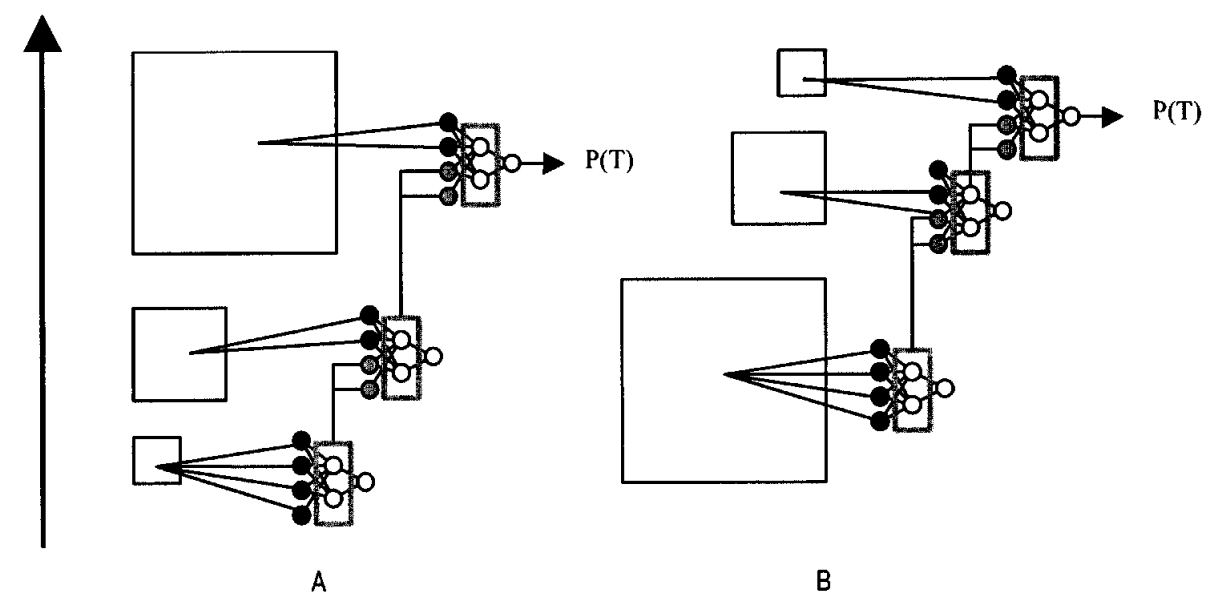
\includegraphics[width=\textwidth]{HPNNarchitecture}
\caption{Hierarchical pyramid/neural network architectures. (A) Coarse-to-fine and (B) fine-to-coarse \cite{sajda2002learning}.}
\label{fig:hpnn}
\end{figure*}

Figure~\ref{fig:hpnn} shows an example architecture of a pyramid neural network. The network shows how the output of one neural network layer feeds into the other along with the lower/higher resolution image input. The output of the higher level layer to the lower layer incurs a dimensionality reduction. This provides the mechanism necessary to cascade the classification of top-level layers to the lower bottom level layers.
\subsection{Convolution}
Convolutional Neural Networks (CNNs) use a connection structure that produces a translation invariant classifier. This is a biologically inspired network that is well suited for image classification. A CNN is connected to its input in such a way that a convolution is applied during classification.  This can be thought of as the neural network scanning the image with a magnifying glass and classifying each component. This is significant as a standard neural network that is trained on a certain input can not handle an input that has been translated. To handle translation in the input the CNN was developed. Since its creation it has been widely used in image classification \cite{6248110,krizhevsky2012imagenet,long2015fully}. CNNs have also shown to be very well suited at classifying complex image datasets such as \cite{deng2009imagenet,Torralba:2008:MTI:1444381.1444403}
\subsection{Hybrid Networks}
A hybrid approach to CNNs and HPNNs is to combine the two approaches in a single deep learning network that is robust to changes in scale as well as translation. Aside from combing just CNNs and HPNNs many deep learning approaches mix fully connected layers and CNNs with HPNNs together to gain accuracy and speed in classification.
\section{Application}
Deep learning networks are widely used in practice and have helped assist medical professionals \cite{sajda2002learning}, classify image datasets \cite{6248110,krizhevsky2012imagenet}, gesture recognition \cite{neverova2014multi}, and drone control and obstacle avoidance \cite{DBLP:journals/corr/ZhangKLA15}.

\subsection{Character Recognition}
\begin{figure}
\centering
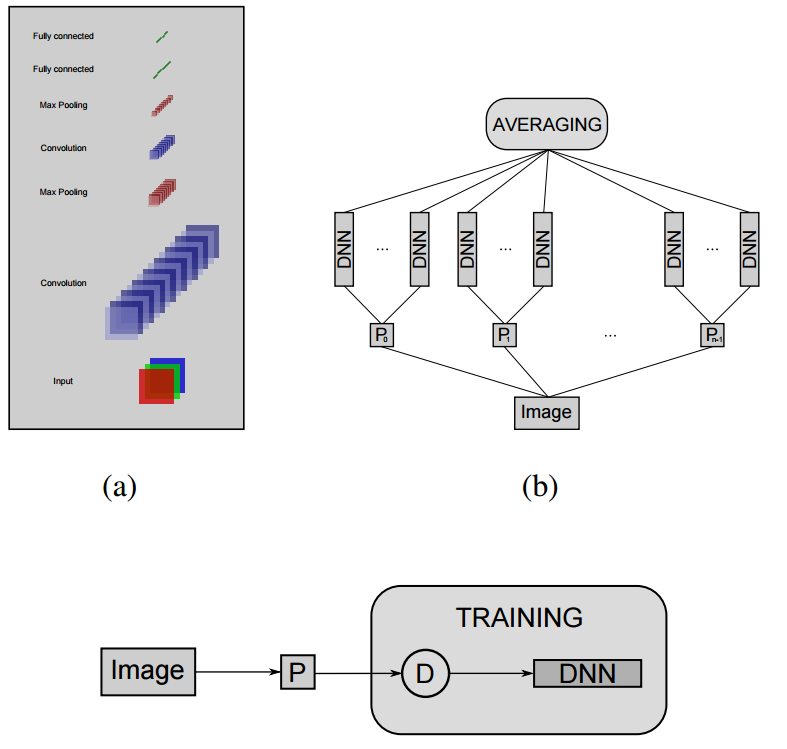
\includegraphics[width=0.4\textwidth]{DNNarchitecture}
\caption{(a) DNN architecture. (b) MCDNN architecture. The input image can be preprocessed by $P_0$ − $P_{n−1}$ blocks. An arbitrary number of columns can be trained on inputs preprocessed in different ways \cite{6248110}.}
\label{fig:multicolumn}
\end{figure}
In \cite{6248110} they train a multi-column Deep Convolutional Neural Network (DNN) on digit classification as well as Chinese characters. This paper introduced a deep neural network that is heavily influenced on the biology of mammalian eyes. The network consists of many columns of DNNs that view different portions of the image. Each columns output is then averaged to get the final output classification. Figure~\ref{fig:multicolumn} shows the architecture of the multi-column DNN classifier. The use of GPUs made the training phase manageable. Instead of taking months to train on a standard CPU using the GPU training times were reduced to a few days.

\subsection{Image Classification}
\begin{figure*}
\centering
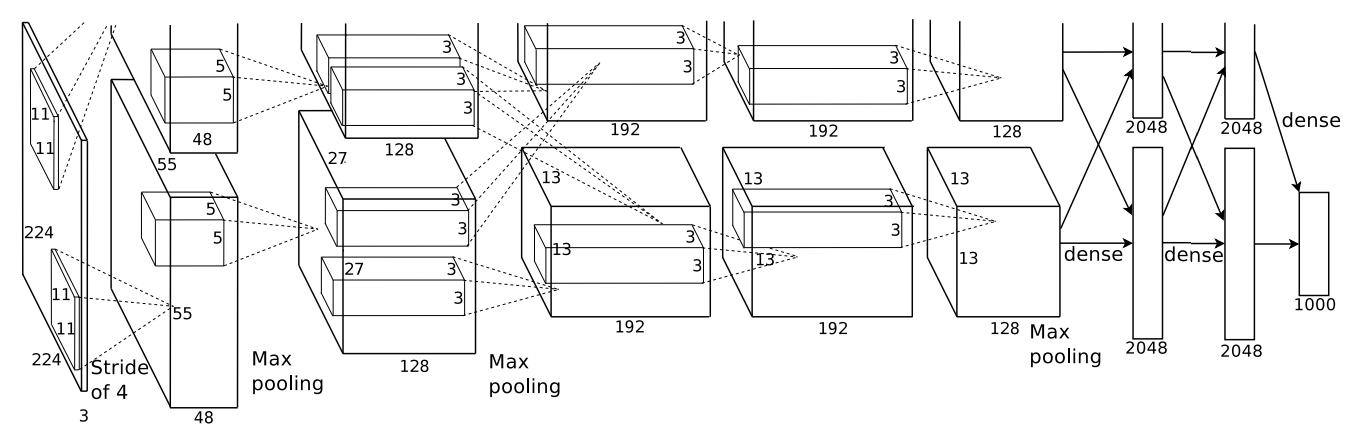
\includegraphics[width=\textwidth]{imagenetarchitecture}
\caption{The architecture of the DNN used in \cite{krizhevsky2012imagenet}. The top half of the network was stored on one GPU while the bottom half was ran on another.}
\label{fig:imagenet}
\end{figure*}
In \cite{krizhevsky2012imagenet} a DNN was used to classify the ImageNet\cite{deng2009imagenet} dataset. The authors were able to improve upon the state of the art by performing the training on GPUs. The architecture of the network was a significant undertaking and took advantage of available hardware. Figure~\ref{fig:imagenet} shows the architecture of the DNN used to train against the ImageNet dataset. The network used was too large to fit in a single GPUs 3GBs of memory. To build a significantly large network two GPUs were used that communicated through SLI. This allowed for parts of the network to train together while others were trained independantly on each individual card.

An interesting component of \cite{krizhevsky2012imagenet} was their method for dealing with overfitting the large network with a large dataset. They combined many data augmentation schemes to increase the input dataset and prevent overfitting of the network. The schemes that were used were used ina way as to prevent further computation of the network.
\subsection{Gesture Recognition}
In \cite{neverova2014multi} deep learning was used to detect and classify gesture recognized from skeleton tracking data from a Kinect sensor. Recognizing gestures is a critical task of robotics as 90\% of communication between people is non-verbal. Recognizing gestures will allow robots to understand human intentions without the need of verbal communication.

\subsection{Obstacle Avoidance}
In \cite{DBLP:journals/corr/ZhangKLA15} a deep neural network was used to train a MPC drone controller to avoid obstacles in real time. This research provides a means to have drones fly in dynamic environments with a monocular camera and avoid collisions with its environment. This was an interesting application of machine learning as I had not heard of such uses of DNNs. The reinforcement learning successfully trained an MPC controller to avoid obstacles in a simulated environment.

\section{Conclusion}
Overall DNNs are a very powerful application of machine learning and have been shown to obtain classification accuracy nearing human levels. These are astonishing results for machine learning. It seems as new strategies arise there are more aspects that machine learning is now able to handle. I plan to use many aspects of machine learning to improve my robotics research. DNN are very powerful, but far more complex that I had anticipated.

\bibliographystyle{IEEEtran}
\bibliography{refs/master}
\end{document}